\documentclass[10pt,a4paper]{article}
\usepackage[utf8]{inputenc}
\usepackage[english]{babel}
\usepackage{amsmath}
\usepackage{amsfonts}
\usepackage{amssymb}
\usepackage{graphicx}
\usepackage[left=2cm,right=2cm,top=2cm,bottom=2cm]{geometry}
\author{Marco Biroli}
\usepackage{physics}
\usepackage{slashed}
\usepackage{stmaryrd}
\title{Master ENS ICFP - First Year 2020/2021\\
Relativistic Quantum Mechanics and Introduction to Quantum Field Theory\\
Mid Term Homework}

\begin{document}
\maketitle

\section[Exercise]{Some operator identities : 6 points}

\begin{enumerate}
\item We have that:
\[
e^A B e^{-A} = \sum_{n = 0}^{\infty} \frac{A^n}{n!} B \sum_{n = 0}^{+\infty} \frac{(-A)^n}{n!} = \sum_{n, m = 0}^{+\infty} \frac{A^n B (-A)^m}{n!m!} = \sum_{n, m = 0}^{+\infty} (-1)^m \frac{A^n B A^m}{n! m!} = \sum_{n = 0}^{+\infty} \frac{A^n}{n!} \sum_{m = 0}^{+\infty} (-1)^m \frac{BA^m}{m!}
\]
...

\item ...

\item We have that:
\[
[F, G^\dagger] = [\sum_j f_j a_j, \sum_j g_j^\star a_j^\dagger] = \sum_{j, k = 0}^{+\infty} f_j g_k^\star [a_j, a_k^\dagger] = \sum_{j, k = 0}^{+\infty} f_j g_k^\star \delta_{jk} = \sum_{j = 0}^{+\infty} f_j g_j^\star
\]
Furthermore we have that $[F, G^\dagger] \propto \text{Id}$ and therefore we trivially have that $[F, [F, G^\dagger]] = [G^\dagger, [F, G^\dagger]] = 0$. Now applying question 2 we have that:
\[
e^{G^\dagger} e^F = e^{-\frac{1}{2} \sum_{j} f_j g_j^\star } e^{G^\dagger + F} \Rightarrow  e^{\frac{1}{2} \sum_{j} f_j g_j^\star }e^F =  \underbrace{e^{\frac{1}{2} \sum_{j} f_j g_j^\star } e^{-\frac{1}{2} \sum_{j} f_j g_j^\star }}_{=e^A e^{-A}} e^{G^\dagger + F}
\]
Now from Question 1 we have that for any $A$ (trivially $[A, \text{Id}] = 0$) we get:
\[
e^A \text{Id} e^{-A} = \text{Id} + \sum_{n=1}^{+\infty} \frac{1}{n!} \cdot 0 = \text{Id}
\]
Hence the above formula simplifies to:
\[
e^{F + G^\dagger} = e^{\frac{1}{2}\sum_j f_jg_j^\star} e^{G^\dagger} e^F
\]

\item Similarly as before let $F = \int \dd^3 \vb{q} f(\vb{q}) a(\vb{q})$ and $G = \int \dd^3 \vb{q} h(\vb{q})^\dagger a(\vb{q})$. Then we have that:
\[
[F, G^\dagger] = [ \int \dd^3 \vb{q} f(\vb{q}) a(\vb{q}), \int \dd^3 \vb{q} h(\vb{q}) a^\dagger(\vb{q})] = \int \dd^3 \vb{q} f(\vb{q})h(\vb{q})[a(\vb{q}), a^\dagger(\vb{q})] = \int \dd^3 \vb{q} f(\vb{q}) h(\vb{q})
\]
A similar direct application of 2 gives the desired result.

\end{enumerate}

\section[Exercise]{An example of an asymptotic series}

We have that:
\[
f(g) = \frac{1}{\sqrt{\pi}} \int_{-\infty}^{+\infty} \dd x e^{-x^2 - g x^4} \mbox{~~hence~~} |f(g)| < \int_{-\infty}^{+\infty} \dd x | e^{-x^2 - g x^4}| = \int_{-\infty}^{+\infty} \dd x e^{-x^2 - x^4 \Re g} < \int_{-\infty}^{+\infty} \dd x e^{-x^4 \Re g}
\]
Hence as long as $\Re g > 0$ this is obviously well defined from the last term and if $\Re g = 0$ this is obviously well defined from the before last term.

\begin{enumerate}
\item This integral admits an exact solution given by:
\[
f(g) = \frac{e^{\frac{1}{8g}} K_{\frac{1}{4}}(\frac{1}{8g})}{2\sqrt{\pi g}} \delta_{\Re g > 0} + \delta_{\Re g = 0} \mbox{~~where~~} K_n(z) \mbox{~~is the modified Bessel function of the second kind.}
\]
The plot of the numerical values for $g \in [0.01, 1]$ is given in Figure \ref{integral:1}.
\begin{figure}
\centering
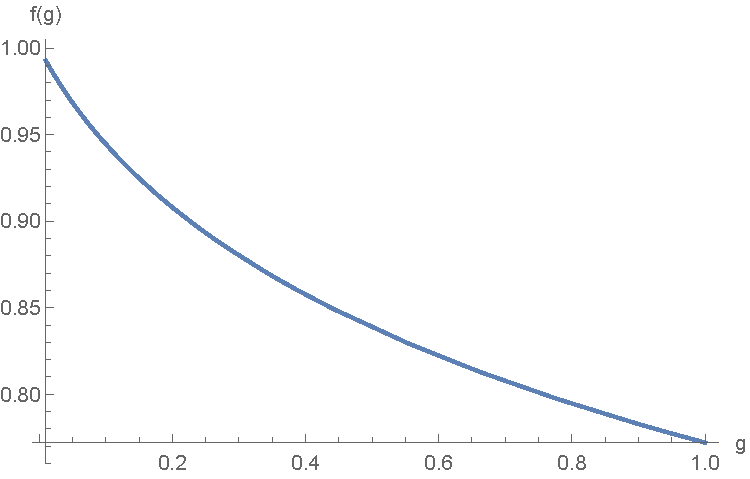
\includegraphics[width = 0.5\textwidth]{integral1}
\caption{Plot of the numerical values of $f(g)$ for $g \in [0.01, 1]$. }\label{integral:1}
\end{figure}
Then $f(g)$ decreases monotonically when $g > 0$ increases since:
\[
\dv{}{g} f(g) = \frac{1}{\sqrt{\pi}} \int_{-\infty}^{+\infty} \dd x (-x^4) e^{-x^2 - g x^4} = \frac{-1}{\sqrt{\pi}} \underbrace{\int_{-\infty}^{+\infty} x^4 e^{-x^2 - g x^4}}_{ > 0 \mbox{~~when~~} g \in \mathbb{R}^+} < 0
\]

\item We have that:
\[
e^{-g x^4} = \sum_{n = 0}^{+\infty} \frac{(-gx^4)^n}{n!}
\]
And plugging this in the expression of $f$ and inverting the sum and the integral gives:
\[
\frac{1}{\sqrt{\pi}} \sum_{n = 0}^{+\infty} \frac{(-g)^n}{n!} \int_{-\infty}^{+\infty} \dd x\,\, x^{4n} e^{-x^2}
\]
We notice the integral ressembles strongly the gamma function hence we change variables by taking $u = x^2$ ($\dd u = 2 \sqrt{u} \dd x$) and we get:
\[
2^{-1} \int_{-\infty}^{+\infty} \dd u u^{2n - \frac{1}{2}} e^{-u} = 2^{-1} \Gamma(2n + \frac{1}{2}) = 2^{-4n} \sqrt{\pi} \frac{\Gamma(4n)}{\Gamma(2n)} \mbox{~~from the Legendre duplication formula.}
\]
Hence plugging it back up top we obtain:
\[
\tilde{f}(g) = \sum_{n = 0}^{+\infty} \left( \frac{(-1)^n(4n)!}{n! 2^{4n} (2n)!} \right) g^n
\]
Notice that the terms $f_n$ are monotonically increasing in norm and diverge hence the sum does not converge absolutely and $R = 0$ and it also does not converge conditionally. The order of magnitude of the first few terms is ...

\item \begin{figure}
\centering
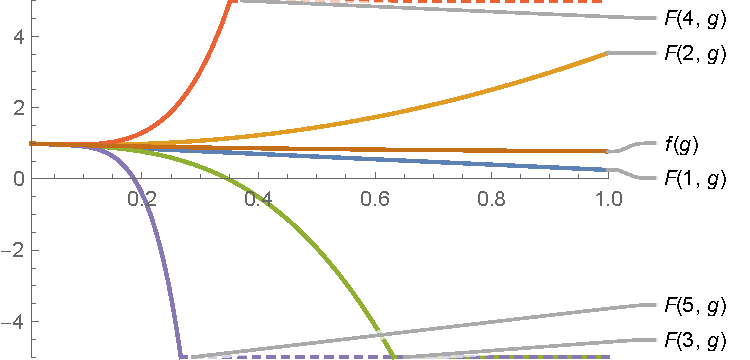
\includegraphics[width=0.44 \textwidth]{approx_series}
\hspace{0.1\textwidth}
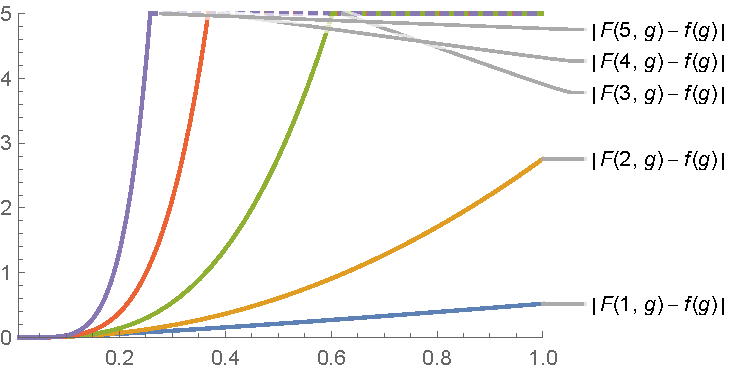
\includegraphics[width=0.44 \textwidth]{error_series}
\caption{Series approximations of $f(g)$ and their errors for $g \in [0.01, 1]$.}
\end{figure}

\end{enumerate}


\section{A relation between Dirac spinors}

\begin{enumerate}

\item Remember that up to a re-writing we have that:
\[
\omega_{ij} = \varepsilon_{i j k} \theta^k \mbox{~~and~~} \omega^{k0} = \nu^k \mbox{~~and~~} \omega_{\mu \nu} = 0 \mbox{~~otherwise.}
\]
Where the $\theta^k$ represent the rotations in the 3 spatial dimensions and the $\nu^k$ represent the boosts along the the three spatial directions. Hence the representation of $L(\vb{p})$ trivially has that $\theta^k = 0$. Then we have that:
\[
i \gamma^0 D(L(\vb{p})) i \gamma^0 = i \gamma^0 \exp( \frac{1}{4} \omega_{\mu \nu} (\gamma^\mu \gamma^\nu - \gamma^\nu \gamma^\mu) ) i \gamma^0
\] 
Now in order to simplify we need to bring the product with the gamma matrices inside. To do so we need to remember two properties. Firstly we have that $(i\gamma^0) = (i\gamma^0)^{-1}$ and secondly we have that: $P e^A P^{-1} = e^{P A P^{-1}}$. Hence applying this formula here we obtain that:
\[
i\gamma^0 D(L(\vb{p})) i \gamma^0 = \exp(\frac{\omega_{\mu \nu}}{4} i\gamma^0 (\gamma^\mu \gamma^\nu - \gamma^\nu \gamma^\mu) i\gamma^0   ) = \exp(\frac{\omega_{\mu \nu}}{4} (i \gamma^0 \gamma^\mu i \gamma^0 i \gamma^0 \gamma^\nu i \gamma^0 - i\gamma^0\gamma^\nu \i \gamma^ 0 i \gamma^0 \gamma^\mu i\gamma^0)   )
\] 
Now we use the formula from the course: $i\gamma^0 \gamma^\mu i \gamma^0 = P^\mu_\nu \gamma^\nu$ where $P^\mu_\nu$ is the parity operator defined in (3.33). Hence this means that the terms in the exponential simplify to:
\[
i\gamma^0 D(L(\vb{p})) i \gamma^0 = \exp(\frac{\omega_{\mu \nu}}{4}  (\gamma^\mu \gamma^\nu - \gamma^\nu \gamma^\mu) (-1)^{1 - \delta^\mu_0}  (-1)^{1 - \delta^\nu_0}) = \exp(\frac{\omega_{\mu \nu}(-1)^{\delta^\mu_0 + \delta^\nu_0 - \delta^\mu_0 \delta^\nu_0} }{4}  (\gamma^\mu \gamma^\nu - \gamma^\nu \gamma^\mu)) 
\]
Hence now we take $\omega'_{\mu \nu} = \omega_{\mu \nu}(-1)^{\delta^\mu_0 + \delta^\nu_0 - \delta^\mu_0 \delta^\nu_0}$, now since $\omega_{00} = 0$ we can discard the term $\delta^\mu_0 \delta^\nu_0$ which means that we are left with:
\[
\omega'_{\mu \nu } = \omega_{\mu \nu}(-1)^{\delta^\mu_0 + \delta^\nu_0} \Leftrightarrow \omega'_{ij} = \omega_{ij} \land \omega'_{k 0} = - \omega_{k 0} \Rightarrow \theta'^k = \theta^k \land \nu'^k = -\nu^k
\]
Hence we have that:
\[
i\gamma^0 D(L(\vb{p})) i \gamma^0 = D(L(-\vb{p}))
\]

\item We have that:
\[
(i p_\mu \gamma^\mu + m) u(\vb{p}, \sigma) = 0 \mbox{~~and~~} (-i p_\mu \gamma^\mu + m) v(\vb{p}, \sigma) = 0
\]
Hence if we take $\vb{p} = 0$ and $p_0 = -p^0 = -m$ for a particle at rest the above simplifies to:
\[
(-im \gamma^0 + m) u(\vb{0}, \sigma) = 0 \mbox{~~and~~} (i m \gamma^0 + m) v(\vb{0}, \sigma) = 0
\]
Which up to dividing by $m$ simplifies to:
\[
(-i \gamma^0 + \vb{1}) u(\vb{0}, \sigma) = 0 \mbox{~~and~~} (i\gamma^0 + \vb{1}) v(\vb{0}, \sigma) = 0
\]
Hence up to a re-writing we have that:
\[
i\gamma^0 u(\vb{0}, \sigma) = u(\vb{0}, \sigma) \mbox{~~and~~} i\gamma^0 v(\vb{0}, \sigma) = - v(\vb{0}, \sigma)
\]
Then from the definition of $u, v$ and $D(L(\vb{p}))$ we have that $u(\vb{p}, \sigma) = D(L(\vb{p})) u(\vb{0}, \sigma)$ and identically for $v$. Hence we have that:
\[
i \gamma^0 u(\vb{p}, \sigma) = i \gamma^0 D(L(\vb{p})) u(\vb{0}, \sigma) = i \gamma^0 D(L(\vb{p})) i \gamma^0 i \gamma^0 u(\vb{0}, \sigma) = D(L(-\vb{p})) u(\vb{0}, \sigma) = u(-\vb{p}, \sigma)
\]
And identically:
\[
i\gamma^0 v(\vb{p}, \sigma) = i\gamma^0 D(L(\vb{p})) v(\vb{0}, \sigma) = i \gamma^0 D(L(\vb{p})) i \gamma^0 i \gamma^0 v(\vb{0}, \sigma) = D(L(-\vb{p})) (-v(\vb{0}, \sigma)) = - v(-\vb{p}, \sigma) 
\]

\end{enumerate}


\section{Some traces of products of $\gamma$-matrices}

We have that:
\[
\tr \gamma_\mu \gamma_\nu = \tr {\gamma_\mu, \gamma_\nu} - \gamma_\nu \gamma_\mu = 2 \tr \eta_{\mu \nu} I_4 - \tr \gamma_\nu \gamma_\mu = 2 \tr \eta_{\mu \nu} I_4 - \tr \gamma_\mu \gamma_\nu
\]
Hence adding on both side we obtain the desired equality:
\[
\tr \gamma_\mu \gamma_\nu = \eta_{\mu \nu} \tr I_4 = 4 \eta_{\mu \nu}
\]
Similarly we have that:
\[
\tr \gamma_\mu \gamma_\nu \gamma_\rho \gamma_\sigma = ... 
\]

\section{Energy levels of a relativistic charged spin-0 particle in a harmonic electrostatic potential}

\begin{enumerate}


\item From these relation we have that:
\begin{align*}
X^2 \ket{n} &= \frac{1}{2 m \Omega} \left( a^2 + (a^\dagger)^2 + \{a, a^\dagger\} \right)\ket{n} \\
&= \frac{1}{2m \Omega} (\sqrt{n}\sqrt{n-1} \ket{n-2} + \sqrt{n+1}\sqrt{n+2} \ket{n+2} + (n+1)\ket{n} + n\ket{n})
\end{align*}
Hence we get that:
\[
\bra{n} X^4 \ket{n} = (\bra{n} X^2)(X^2 \ket{n}) = \frac{1}{(2 m \Omega)^2} (n^2 - n + n^2 + 3n + 2 + n + 1 + n) = \frac{2n^2 + 3n + 2}{(2m \Omega)^2}
\]

\item We have that:
\[
(D_\mu D^\mu + m^2) \Phi = 0 \mbox{~~where~~} D^\mu = \partial^\mu - i q A^\mu
\]
Then taking $\Phi = e^{- i E t} \phi$ and plugging it in we get that:
\[
e^{-iEt} (D_i D^i + m^2) \phi + D_0D^0 e^{-iE t} \phi = 0
\]
Looking now only at the second term we have that:
\[
D_0D^0 e^{-iE t} \phi = (\partial_0 + i\frac{m}{2}\omega^2 x^2)(\partial^0 - i \frac{m}{2} \omega^2 x^2) e^{- i E t}\phi = (\partial_0 \partial^0 + \frac{m}{2} \omega^2 x^2) e^{-i E t} \phi = 
\]
Now looking at the time derivative we obtain:
\[
\partial_0\partial^0 e^{-iE t}\phi = \partial_0 (-i E e^{-iEt}\phi + e^{-iEt}\partial^0\phi) = E^2 e^{-iEt} \phi - i E e^{-iEt} \partial^0 \phi + e^{-iEt}\partial_0\partial^0 \phi 
\]

\item 

\end{enumerate}

\section{The axial current}

\begin{enumerate}

\item We know that $\{\gamma_5, \gamma^\mu\} = 0$ and hence $\gamma_5 \gamma^\mu = - \gamma^\mu \gamma_5$. Then we have that:
\[
e^{i \varepsilon \gamma_5} \gamma^\mu = \sum_{n \in \mathbb{N}} \frac{1}{n!} (i \varepsilon \gamma_5)^n \gamma^\mu = \sum_{n \in \mathbb{N}} \frac{1}{n!} (-1)^n \gamma^\mu (i \varepsilon \gamma_5)^n  = \gamma^\mu \sum_{n \in \mathbb{N}} \frac{(-i \varepsilon \gamma_5)^n}{n!} = \gamma^\mu e^{- i \varepsilon \gamma_5}
\]
Notice also trivially that $(e^{i \varepsilon\gamma_5})^\dagger = e^{- i \varepsilon \gamma_5}$ since $\gamma_5 = \gamma_5^\dagger$. Hence the axial transformation gives:
\[
\overline{e^{i \varepsilon \gamma_5}\psi} = (e^{i\varepsilon \gamma_5} \psi)^\dagger i \gamma^0 = \psi^\dagger e^{- i \varepsilon \gamma_5} i \gamma^0 = \psi^\dagger i \gamma^0 e^{i\varepsilon \gamma_5} = \overline{\psi} e^{i \varepsilon \gamma_5}
\]

\item If we replace $\psi$ by the axial transformed $e^{i \varepsilon \gamma_5} \psi$ we also have to replace $\overline{\psi}$ by the axial transformed $\overline{\psi} e^{i \varepsilon \gamma_5}$. Hence we obtain:
\[
S = \int \dd^4 x \overline{\psi} e^{i \varepsilon\gamma_5} (- \slashed{\partial}  + i q \slashed{A} - m) e^{i\varepsilon\gamma_5} \psi
\]
Now notice that:
\[
e^{i\varepsilon\gamma_5} \slashed{a} e^{i\varepsilon \gamma_5} = e^{i\varepsilon \gamma_5} a_\mu \gamma^\mu e^{i\varepsilon \gamma_5} = (a_\mu e^{i\varepsilon \gamma_5} + [e^{i\varepsilon \gamma_5}, a_\mu]) \gamma^\mu e^{i\varepsilon \gamma_5} = a_\mu + [e^{i\varepsilon \gamma_5}, a_\mu] \gamma^\mu e^{i\varepsilon \gamma_5}
\]
Then since $[\partial_\mu, e^{i\varepsilon \gamma_5}] = 0$ and $[A_\mu, e^{i\varepsilon \gamma_5}] = 0$ we have that:
\[
S = \int \dd^4 x \overline{\psi}(-\slashed{\partial} + i q \slashed{A} - m e^{i2\varepsilon \gamma_5}) \psi
\]
Hence the action is left unchanged if and only if $m = 0$ or $\varepsilon = 0$. The second case corresponding to the trivial case of reducing the transformation to the identity can be discarded. Now assuming $m = 0$. The infinitesimal transformation corresponding to the axial transformation is given by:
\[
\psi \longmapsto e^{i \varepsilon \gamma_5} \psi = (1 + i \varepsilon \gamma_5) \psi = \psi + i\varepsilon \gamma_5 \psi
\]
Now this transformation conserves both the action and the Lagrangian hence from the formula (4.53) of the notes we have that the corresponding conserved current is given by:
\[
j_5^\mu = - \pdv{\mathcal{L}}{\partial_\mu \psi^a}\pdv{\psi^a}{\varepsilon} = - i \overline{\psi} \gamma^\mu  \gamma_5 \psi 
\]

\item The Dirac equations are given by:
\[
(\slashed{\partial} - i q \slashed{A} + m) \psi = 0 \mbox{~~and~~} \overline{\psi}(- \overleftarrow{\slashed{\partial}} + i q \slashed{A} + m) = 0 
\] 
Then we have that:
\[
\partial_\mu j_5^\mu = \partial_\mu (-i \overline{\psi} \gamma^\mu \gamma_5 \psi) = - \overline{\psi}( \slashed{\partial} + \overleftarrow{\slashed{\partial}} ) \gamma_5 \psi = - \overline{\psi}( i q \slashed{A} - m - i q \slashed{A} - m)\gamma_5 \psi = 2m \overline{\psi}\gamma_5 \psi \propto m 
\]
\end{enumerate}

\section{Supersymmetry}

\begin{enumerate}

\item 

\end{enumerate}

\end{document}